% ============================================================
% 第三章 第3.2节：状态依赖自适应协同（SDAS）模型的
%              软件实现与仿真验证
% 编译方式：xelatex → xelatex（需两次编译）
% ============================================================
\documentclass[12pt,a4paper]{report}

% ---- 中文支持 ----
\usepackage{fontspec}
\usepackage{xeCJK}
\setCJKmainfont{SimSun}
\setCJKsansfont{SimHei}
\setCJKmonofont{FangSong}

% ---- 数学公式 ----
\usepackage{amsmath,amssymb}

% ---- 代码片段 ----
\usepackage{listings}
\lstset{
    basicstyle=\ttfamily\small,
    numbers=left,
    numberstyle=\tiny,
    frame=single,
    breaklines=true,
    language=Python,
    captionpos=b,
    tabsize=4,
    showstringspaces=false,
}

% ---- 算法环境 ----
\usepackage{algorithm}
\usepackage{algpseudocode}

% ---- 图片 ----
\usepackage{graphicx}
\usepackage{caption}
\usepackage{subcaption}
\graphicspath{{./figures/}}

% ---- 表格 ----
\usepackage{booktabs}
\usepackage{array}
\usepackage{multirow}

% ---- 引用与交叉引用 ----
\usepackage[colorlinks=true, linkcolor=black, citecolor=black]{hyperref}

% ---- 页面设置 ----
\usepackage{geometry}
\geometry{left=2.5cm,right=2.5cm,top=2.5cm,bottom=2.5cm}
\usepackage{setspace}
\linespread{1.3}

% ---- 符号宏 ----
\newcommand{\R}{\mathbb{R}}
\newcommand{\E}{\mathbf{E}}
\newcommand{\q}{\mathbf{q}}
\newcommand{\T}{\mathsf{T}}

\begin{document}

\setcounter{section}{3}
\setcounter{subsection}{1}

\subsection{状态依赖自适应协同（SDAS）模型的软件实现与仿真验证}
\label{sec:sdas_implementation}

本节基于第\,\ref{sec:sdas_theory} 节建立的 SDAS 理论框架，系统地介绍该模型在 Python 编程环境中的完整软件实现，并通过两类数值仿真——运动学交互仿真与动力学数值仿真——对模型的核心性质进行验证。在进入具体实现细节之前，本节首先概述软件系统的整体架构与数据流。


\subsubsection{软件架构与数据流}
\label{sec:architecture}

本文开发的折纸手仿真工具包 \lstinline{synergy\_hand\_sim} 在功能上涵盖从 CAD 设计到交互式三维物理仿真的完整流程。就 SDAS 模型而言，其核心计算链路由以下五个功能层次组成：

\begin{enumerate}
    \item \textbf{解析层}：负责加载 \lstinline{.ohd} 格式的折纸手设计文件，通过 \lstinline{OrigamiHandDesign.load()} 将 JSON 序列化的几何与拓扑信息反序列化为内存中的设计对象。
    \item \textbf{数据模型层}：以 \lstinline{OrigamiHandDesign} 类为核心容器，管理折痕线（\lstinline{fold\_lines}）、面片（\lstinline{faces}）、滑轮（\lstinline{pulleys}）、孔（\lstinline{holes}）、腱绳路径（\lstinline{tendons}）和驱动器（\lstinline{actuators}）等全部设计数据。
    \item \textbf{协同层}：即 \lstinline{SDASModel} 类。在构造阶段接收传动向量 $\mathbf{R}_A$ 和 $\mathbf{R}_B$，预计算所有系数矩阵；在运行阶段接收电机位移输入，输出满足传动约束的关节角度向量。
    \item \textbf{仿真层}：包含两套并行的仿真机制。\textbf{运动学交互仿真器}基于 MuJoCo 物理引擎，通过滑块回调接口实时驱动三维模型；\textbf{动力学数值仿真器}由 \lstinline{HandSimulator} 类封装，包含惯性与阻尼模型，通过 ODE 积分输出关节角度的时间历程。
    \item \textbf{可视化层}：MuJoCo 原生 GLFW 查看器提供三维渲染，滑块面板提供交互控制；动力学仿真的结果通过 \lstinline{SimulationVisualizer} 生成 q(t) 曲线等多面板图表。
\end{enumerate}

SDAS 模型在这两种仿真中均扮演``关节角度生成器''的角色。在运动学交互仿真中，求解链路为 $\lstinline{.ohd} \to \mathbf{R}_A/\mathbf{R}_B \to \lstinline{SDASModel} \to \lstinline{synergy\_callback} \to \lstinline{qpos} \to \lstinline{mj\_forward} \to \text{渲染}$。该链路仅在程序启动时进行一次模型初始化，运行时每帧仅执行一次 \lstinline{solve\_motors()} 求解和 \lstinline{qpos} 赋值。在动力学数值仿真中，链路扩展为 $\lstinline{.ohd} \to \mathbf{R}_A/\mathbf{R}_B + \text{惯性/刚度/阻尼参数} \to \text{动力学方程装配} \to \text{ODE 积分器} \to \text{轨迹输出}$。SDAS 模型在动力学仿真中生成 $\sigma(t)$ 和 $\sigma_f(t)$ 对应的参考关节角度序列，该序列作为弹性恢复力的参考构型输入到动力学方程中。

两套仿真机制的根本区别在于是否考虑惯性和阻尼。运动学交互仿真仅计算静力平衡下的关节角度，不涉及时间演化；动力学数值仿真则在 $\sigma$ 和 $\sigma_f$ 发生阶跃变化时，能够输出关节角度随时间连续过渡的动态响应，这对验证 SDAS 模型在真实物理环境中的动态行为至关重要。


\subsubsection{核心数据结构：OrigamiHandDesign}
\label{sec:data_structures}

SDAS 模型软件实现的数据基础是 \lstinline{OrigamiHandDesign} 类（见 \lstinline{src/models/origami_design.py}）。该类的设计遵循``数据与算法分离''原则——类本身仅负责存储和查询，不涉及传动矩阵计算或运动学求解等算法逻辑。与 SDAS 模型密切相关的成员字段及其含义列于表\,\ref{tab:design_fields}。

\begin{table}[htbp]
\centering
\caption{\lstinline{OrigamiHandDesign} 中与 SDAS 模型密切相关的关键属性}
\label{tab:design_fields}
\small
\begin{tabular}{@{}p{2.5cm}p{2.5cm}p{8.5cm}@{}}
\toprule
\textbf{字段} & \textbf{数据类型} & \textbf{说明} \\
\midrule
\lstinline{fold_lines} & \lstinline{dict[int, FoldLine]} & 所有折痕线字典。每个 \lstinline{FoldLine} 包含起止点坐标、折痕类型（\lstinline{MOUNTAIN} / \lstinline{VALLEY} / \lstinline{OUTLINE}）和弯曲刚度系数 $\kappa_i$。每个活动关节对应一条折痕线。\\
\lstinline{faces} & \lstinline{dict[int, OrigamiFace]} & 面片字典。每个面片由顶点序列和边 ID 序列定义，用于 URDF 导出和碰撞检测网格生成。\\
\lstinline{joints} & \lstinline{list[JointConnection]} & 关节连接表。每条记录包含关联的折痕线 ID、两个面片 ID 和折痕类型，描述相邻面片间的转动自由度。\\
\lstinline{pulleys} & \lstinline{dict[int, Pulley]} & 滑轮字典。滑轮 ID 为正整数，包含位置、半径 $r$、摩擦系数 $\mu$ 和附着折痕 ID。\\
\lstinline{holes} & \lstinline{dict[int, Hole]} & 孔字典。孔 ID $\le -100$，包含位置、板厚偏移 $h$、摩擦系数 $\mu$ 和附着折痕 ID。\\
\lstinline{tendons} & \lstinline{dict[int, Tendon]} & 腱绳路径字典。记录元素 ID 序列：正数为滑轮，$-1$ 为驱动器 A，$-2$ 为驱动器 B，$\le -100$ 为孔。\\
\lstinline{actuators} & \lstinline{dict[int, Actuator]} & 驱动器字典。预定义两个驱动器，ID 分别为 $-1$（Motor A）和 $-2$（Motor B）。\\
\bottomrule
\end{tabular}
\end{table}

关节索引的获取通过 \lstinline{get_joint_list()} 函数完成。该函数位于 \lstinline{src/models/transmission_builder.py}，其返回值包含两个元素：按 ID 排序的 \lstinline{JointConnection} 列表，以及 \lstinline{fold\_line\_id} 到关节索引的映射字典。当设计尚未重建拓扑时，函数直接从 \lstinline{fold_lines} 中筛选谷折和山折类型的折痕线作为关节，从而保留原始的 \lstinline{fold\_line\_ID}，使滑轮和孔中记录的 \lstinline{attached\_fold\_line\_id} 与关节索引之间的映射关系不断裂。

从 SDAS 模型的角度来看，腱绳路径的拓扑结构是最关键的信息。以表\,\ref{tab:design_fields} 中的 \lstinline{tendons} 字段为例，一条包含元素序列 $[e_0, e_1, \dots, e_{N-1}]$ 的腱绳中，$e_0 = -1$（Motor A）、$e_{N-1} = -2$（Motor B），中间元素为滑轮或孔。该序列唯一确定了从两台驱动器出发的 Capstan 张力衰减路径，从而决定了 $\mathbf{R}_A$ 与 $\mathbf{R}_B$ 两个传动向量的分布。


\subsubsection{单侧传动矩阵 $\mathbf{R}_A$ 与 $\mathbf{R}_B$ 的计算}
\label{sec:RA_RB_computation}

传动矩阵 $\mathbf{R}_A$ 和 $\mathbf{R}_B$ 的计算是 SDAS 模型区别于经典自适应协同模型的核心环节。在经典自适应协同中，传动矩阵 $\mathbf{R}$ 被视为固定常数矩阵，物理上隐含了腱绳两端张力相等同时作用的假设。然而，真实的绳驱系统中，由于 Capstan 摩擦使张力沿路径指数衰减，两端驱动器的张力分布并不相同。

\paragraph{物理模型}

由第\,\ref{sec:sdas_theory} 节中的式\,(2.23) 和\,(2.25) 可知，当驱动器 A 输入张力 $F_A$ 时，传播至第 $j$ 个导向元件时的衰减因子为 $\alpha_j^{(A)} = \exp(-\sum_{k \in \mathcal{P}_A(j)} \beta_k)$，其中 $\beta_k = \mu_k\theta_k$ 为第 $k$ 个导向元件的有效摩擦系数。类似地，从驱动器 B 出发有 $\alpha_j^{(B)} = \exp(-\sum_{k \in \mathcal{P}_B(j)} \beta_k)$。在实用中取所有 $\beta_k \equiv \beta$，则对于第 $j$ 个元素有 $\alpha_j^{(A)} = e^{-\beta j}$ 和 $\alpha_j^{(B)} = e^{-\beta (N-1-j)}$，其中 $N$ 为路径元素总数。

参数 $\beta$ 的默认值为 $\beta = 0.09$。该取值的物理含义是：单个导向元件导致的张力衰减约为 $1 - e^{-0.09} \approx 8.6\%$。经过 42 个导向元件后，张力衰减至初始值的 $e^{-0.09 \times 42} \approx 0.023$，即约 2.3\%。

由第\,\ref{sec:sdas_theory} 节中的式\,(2.30) 可知，$\mathbf{R}_A$ 和 $\mathbf{R}_B$ 的第 $i$ 个分量为附着于关节 $i$ 的所有导向元件的半径 $r_k$ 经衰减加权后的累加和：
\begin{align}
    R_A[i] &= \sum_{k \in \mathcal{J}_i} r_k \cdot e^{-\beta \cdot d_A(k)}, \label{eq:RA_impl}\\
    R_B[i] &= \sum_{k \in \mathcal{J}_i} r_k \cdot e^{-\beta \cdot d_B(k)}, \label{eq:RB_impl}
\end{align}
其中 $\mathcal{J}_i$ 为附着于关节 $i$ 的所有导向元件集合，$d_A(k)$ 和 $d_B(k)$ 分别为元素 $k$ 到驱动器 A 和 B 沿路径的步数。

\paragraph{代码实现}

函数 \lstinline{compute_R_one_sided()} 实现了上述计算。其核心循环遍历每条腱绳路径上的每个导向元件，对每个元件获取其半径和所附着的关节索引，然后按式\,\eqref{eq:RA_impl}--\eqref{eq:RB_impl} 累加传动比。以下为该函数的核心代码：

\begin{lstlisting}[language=Python, caption=\lstinline{compute_R_one_sided()} 的核心循环]
def compute_R_one_sided(design, beta=0.09):
    joints, jid_to_idx = get_joint_list(design)
    n = len(joints)
    R_A_list, R_B_list = [], []

    for tendon in design.tendons.values():
        elements = [eid for eid in tendon.pulley_sequence
                    if eid >= 0 or is_hole_id(eid)]
        N = len(elements)
        row_A, row_B = np.zeros(n), np.zeros(n)

        for k, eid in enumerate(elements):
            r = get_element_radius(eid, design)     # 滑轮半径或孔偏移
            if r <= 0:
                continue
            j_idx = get_element_joint_idx(eid, design, jid_to_idx)
            if j_idx is None:
                continue

            d_A = float(k)                          # 到 Motor A 的步数
            d_B = float(N - 1 - k)                  # 到 Motor B 的步数
            w_A = np.exp(-beta * d_A)
            w_B = np.exp(-beta * d_B)

            row_A[j_idx] += r * w_A
            row_B[j_idx] += r * w_B

        R_A_list.append(row_A)
        R_B_list.append(row_B)

    R_A = np.array(R_A_list)
    R_B = np.array(R_B_list)
    return R_A, R_B
\end{lstlisting}

计算中有两点需说明。第一，\lstinline{get_element_radius()} 对滑轮返回其 \lstinline{radius} 字段，对孔则返回 \lstinline{plate_offset} 字段——孔的等效半径由折纸板的厚度决定。第二，当存在多条驱动腱绳时，函数 \lstinline{build_sdas_model()} 会取所有驱动腱绳的算术平均作为最终的 $\mathbf{R}_A$ 和 $\mathbf{R}_B$，这是因为所有腱绳共享相同的驱动器 A 和 B，平均传动向量共同决定系统的宏观传动行为。

以下为计算过程的算法伪代码：

\begin{algorithm}[htbp]
\caption{单侧传动矩阵 $\mathbf{R}_A$ 与 $\mathbf{R}_B$ 的计算}
\label{alg:compute_RA_RB}
\begin{algorithmic}[1]
\Require 折纸设计 \lstinline{design}，有效摩擦系数 $\beta$
\State 提取关节列表并建立 \lstinline{fold_line_id} $\to$ 关节索引映射 $\mathcal{M}$
\State 初始化 $\mathcal{R}_A \gets []$，$\mathcal{R}_B \gets []$
\For{each 腱绳 $t \in$ \lstinline{design.tendons}}
    \State 过滤出导向元件序列 $\mathcal{E} = [e_0, e_1, \dots, e_{N-1}]$
    \State $\tilde R_A \gets \mathbf{0} \in \R^{n}$，$\tilde R_B \gets \mathbf{0} \in \R^{n}$
    \For{$j \gets 0$ \textbf{to} $N-1$}
        \State $r \gets$ \lstinline{get_element_radius($e_j$)}
        \State $i \gets \mathcal{M}$\lstinline{.get(get_fold_id($e_j$))}
        \If{$i \neq \text{None}$}
            \State $\tilde R_A[i] \gets \tilde R_A[i] + r \cdot e^{-\beta j}$
            \State $\tilde R_B[i] \gets \tilde R_B[i] + r \cdot e^{-\beta (N-1-j)}$
        \EndIf
    \EndFor
    \State 将 $\tilde R_A$、$\tilde R_B$ 分别添加至 $\mathcal{R}_A$、$\mathcal{R}_B$
\EndFor
\State 仅保留驱动腱绳对应的行，对多条驱动腱绳取平均
\Return $(\mathbf{R}_A, \mathbf{R}_B)$
\end{algorithmic}
\end{algorithm}

算法\,\ref{alg:compute_RA_RB} 的计算复杂度为 $\mathcal{O}(N_t \cdot N_e)$，其中 $N_t$ 为腱绳数量，$N_e$ 为每条腱绳的导向元件数量。典型的三指折纸手设计（1 条驱动腱绳、约 40 个导向元件）单次计算耗时约 0.1\,ms。


\subsubsection{SDAS 模型类的实现}
\label{sec:sdas_class}

SDAS 的约束求解器封装在 \lstinline{SDASModel} 类中（见 \lstinline{src/synergy/sdas_model.py}）。构造函数接收四个参数：关节数量 $n$、行向量 $\mathbf{R}_A \in \R^{1 \times n}$、行向量 $\mathbf{R}_B \in \R^{1 \times n}$ 以及关节刚度向量 $\mathbf{E}_{\text{vec}} \in \R^{n}$。

\paragraph{预计算}

在构造阶段，首先建立对角刚度矩阵 $\mathbf{E} = \operatorname{diag}(\mathbf{E}_{\text{vec}})$ 及其逆 $\mathbf{E}^{-1} = \operatorname{diag}(1/\mathbf{E}_{\text{vec}})$。

由第\,\ref{sec:sdas_theory} 节中的式\,(2.40)--(2.41) 可知，Schur 补求解需要先计算三个标量系数：
\begin{align}
    a &= \mathbf{R}_A \mathbf{E}^{-1} \mathbf{R}_A^{\mathsf{T}}, \nonumber\\
    b &= \mathbf{R}_A \mathbf{E}^{-1} \mathbf{R}_B^{\mathsf{T}}, \nonumber\\
    c &= \mathbf{R}_B \mathbf{E}^{-1} \mathbf{R}_B^{\mathsf{T}}, \label{eq:schur_scalars}\\
    \Delta &= a c - b^2. \label{eq:schur_det}
\end{align}
当 $\Delta < 10^{-15}$ 时系统退化，此时 $\mathbf{R}_A$ 与 $\mathbf{R}_B$ 线性相关，通常出现在对称路径且刚度均匀的条件下。构造函数中对此进行检查并给出警告。

随后通过式\,(2.39) 提取出 $\mathbf{S}_A$ 和 $\mathbf{S}_B$ 的系数向量：
\begin{align}
    \mathbf{S}_A^{\text{(schur)}} &= \mathbf{E}^{-1}\big(c \mathbf{R}_A^{\mathsf{T}} - b \mathbf{R}_B^{\mathsf{T}}\big) / \Delta, \label{eq:schur_SA}\\
    \mathbf{S}_B^{\text{(schur)}} &= \mathbf{E}^{-1}\big(-b \mathbf{R}_A^{\mathsf{T}} + a \mathbf{R}_B^{\mathsf{T}}\big) / \Delta. \label{eq:schur_SB}
\end{align}
同步预计算单马达单向公式的系数向量：
\begin{align}
    \mathbf{S}_A^{\text{(paper)}} &= \mathbf{E}^{-1} \mathbf{R}_A^{\mathsf{T}} / a, \label{eq:paper_SA}\\
    \mathbf{S}_B^{\text{(paper)}} &= \mathbf{E}^{-1} \mathbf{R}_B^{\mathsf{T}} / c. \label{eq:paper_SB}
\end{align}
以及外力柔顺矩阵 $\mathbf{C}$。

以下为构造函数的简要实现代码：

\begin{lstlisting}[language=Python, caption=SDASModel 构造函数的预计算逻辑]
class SDASModel:
    def __init__(self, n_joints, R_A, R_B, E_vec):
        self.n_joints = n_joints
        self.R_A, self.R_B = R_A.copy(), R_B.copy()
        self.E = np.diag(E_vec)
        self.E_inv = np.diag(1.0 / E_vec)

        a = float(self.R_A @ self.E_inv @ self.R_A.T)
        b = float(self.R_A @ self.E_inv @ self.R_B.T)
        c = float(self.R_B @ self.E_inv @ self.R_B.T)
        self.det = a * c - b * b

        # Schur 补系数（双马达模式）
        self.S_A_schur = self.E_inv @ (R_A.T * c - R_B.T * b) / self.det
        self.S_B_schur = self.E_inv @ (-R_A.T * b + R_B.T * a) / self.det

        # 单向公式系数（单马达模式）
        self.S_A_paper = self.E_inv @ R_A.T / a
        self.S_B_paper = self.E_inv @ R_B.T / c
\end{lstlisting}

\paragraph{核心求解方法}

\lstinline{solve_motors()} 是低层求解接口，其核心逻辑由四个分支组成（见算法\,\ref{alg:solve_motors}）。首先对 $\theta_A$ 和 $\theta_B$ 执行松弛钳位（负位移置零），然后根据激活状态选择求解公式。

\begin{algorithm}[htbp]
\caption{\lstinline{solve_motors()} 的约束选择逻辑}
\label{alg:solve_motors}
\begin{algorithmic}[1]
\Require 电机输入 $\theta_A$, $\theta_B$，阈值 $\varepsilon = 10^{-10}$
\Require 可选：雅可比矩阵 $\mathbf{J}$，外力 $\mathbf{f}_{\text{ext}}$
\Ensure 关节角 $\mathbf{q} \in \R^n$
\State $\theta_A \gets \max(0, \theta_A)$，$\theta_B \gets \max(0, \theta_B)$ \Comment{松弛钳位}
\If{$\theta_A > \varepsilon$ \textbf{and} $\theta_B > \varepsilon$}
    \State $\mathbf{q} \gets \mathbf{S}_A^{\text{(schur)}} \theta_A + \mathbf{S}_B^{\text{(schur)}} \theta_B$
\ElsIf{$\theta_A > \varepsilon$}
    \State $\mathbf{q} \gets \mathbf{S}_A^{\text{(paper)}} \theta_A$
\ElsIf{$\theta_B > \varepsilon$}
    \State $\mathbf{q} \gets \mathbf{S}_B^{\text{(paper)}} \theta_B$
\Else
    \State $\mathbf{q} \gets \mathbf{0}$
\EndIf
\If{外力信息存在且非零}
    \State $\mathbf{q} \gets \mathbf{q} + \mathbf{C} \mathbf{J}^{\mathsf{T}} \mathbf{f}_{\text{ext}}$
\EndIf
\Return $\mathbf{q}$
\end{algorithmic}
\end{algorithm}

\lstinline{solve_synergies()} 是高层接口，接收协同变量 $\sigma$（共模分量）和 $\sigma_f$（差模分量）作为输入。由第\,\ref{sec:sdas_theory} 节中电机位移与协同变量的关系可知，二者满足：
\begin{equation}
    \theta_A = \max(0, \sigma + \sigma_f),\quad \theta_B = \max(0, \sigma - \sigma_f),
    \label{eq:sigma_to_theta}
\end{equation}
其中 $\sigma \ge 0$。由于 \lstinline{solve_motors()} 内部已包含松弛钳位，当 $|\sigma_f| > \sigma$ 时 $\theta_B$ 或 $\theta_A$ 被自动钳位为零，系统退化为单马达模式。这种切换准确反映了物理世界中腱绳松弛侧不再传递驱动力的行为。


\subsubsection{MuJoCo 交互仿真器集成}
\label{sec:mujoco_integration}

交互式仿真环境是检验 SDAS 模型实时性能和验证行为合理性的重要工具。系统通过 \lstinline{scripts/run_synergy_from_ohd.py} 脚本启动，其工作流程分为构建与运行两个阶段。

\paragraph{构建阶段}

程序启动时依次执行以下步骤：(i) 加载 \lstinline{.ohd} 文件；(ii) 调用 \lstinline{build_sdas_model()} 构建 SDAS 模型——其间依次执行关节提取、$\mathbf{R}_A/\mathbf{R}_B$ 计算和 \lstinline{SDASModel} 构造；(iii) 通过空间最近邻匹配建立 URDF 关节名称与协同模型关节索引的映射关系——该算法将每个 URDF 铰链关节的全局坐标与所有折痕线中点进行距离比对，取最近匹配；(iv) 启动 \lstinline{MuJoCoSimulator}，传入协同回调函数。

\paragraph{运行时的滑块回调机制}

MuJoCo 仿真器右侧面板包含四个滑块，分别对应 Motor A 位移、Motor B 位移、共模协同变量 $\sigma$ 和差模协同变量 $\sigma_f$。滑块之间具有互联动功能，由以下逻辑实现：

\begin{enumerate}
    \item 比较当前帧 \lstinline{data.ctrl} 与上一帧 \lstinline{prev_ctrl} 的差值。若 A/B 滑块变化量主导，则通过式\,\eqref{eq:sigma_to_theta} 的逆映射 $\sigma = (\theta_A + \theta_B)/2$、$\sigma_f = (\theta_A - \theta_B)/2$ 更新 $\sigma$/$\sigma_f$ 滑块。
    \item 若 $\sigma$/$\sigma_f$ 滑块变化量主导，则通过式\,\eqref{eq:sigma_to_theta} 的正向映射计算 $\theta_A/\theta_B$ 并更新 A/B 滑块。
    \item 若两种变化量均小于容差，保持上次互联动主从关系不变。
\end{enumerate}

回调函数的简化代码如下：

\begin{lstlisting}[language=Python, caption=仿真器协同回调函数的核心逻辑]
def synergy_callback(theta1_rad, theta2_rad, speed_rad_s=0.0):
    # Slack 钳位
    theta_A = max(0.0, float(theta1_rad))
    theta_B = max(0.0, float(theta2_rad))

    # SDAS 求解（内部自动选择公式）
    q = sdas_model.solve_motors(theta_A, theta_B)

    # 限位并组装结果
    result = {}
    for urdf_name, syn_idx in urdf_to_syn_map.items():
        if 0 <= syn_idx < len(q):
            raw_angle = q[syn_idx]
            fold_type = syn_idx_to_fold_type.get(syn_idx)
            clamped = clamp_fold_angle(raw_angle, fold_type) \
                      if fold_type is not None else raw_angle
            result[urdf_name] = clamped
        else:
            result[urdf_name] = 0.0
    return result
\end{lstlisting}

该回调在 MuJoCo 主循环每帧被调用一次。对于典型设计（10 个关节），单次 \lstinline{solve_motors()} 耗时约 2--5\,$\mu$s，加上限位处理和结果字典组装后总耗时约 10--20\,$\mu$s，远小于 MuJoCo 引擎自身的步进耗时（约 1--5\,ms），因此 SDAS 模型的引入不会对交互帧率造成可感知的影响。


\subsubsection{仿真验证与结果分析}
\label{sec:simulation_validation}

为验证 SDAS 模型的正确性和物理合理性，本节进行三组数值实验。所有实验均采用 \lstinline{models/ohd test/ohd_2.ohd} 三指折纸手设计，其参数列于表\,\ref{tab:validation_params}。

\begin{table}[htbp]
\centering
\caption{仿真验证实验的基本参数配置}
\label{tab:validation_params}
\small
\begin{tabular}{@{}lcl@{}}
\toprule
\textbf{参数} & \textbf{值} & \textbf{说明} \\
\midrule
关节总数 & 10 & 全部为谷折型折痕 \\
驱动腱绳数量 & 1 & 串联所有手指 \\
关节刚度 $\mathbf{E}$ & $\mathbf{I}$ & 单位刚度，不计外力 \\
Capstan 摩擦系数 $\beta$ & 0.09 & 默认值 \\
运动学仿真 & 直接求解 & SDASModel.solve\_motors() \\
动力学仿真 & Phase 2 & RK4 积分器，$dt = 10^{-4}\,\text{s}$ \\
\bottomrule
\end{tabular}
\end{table}

\paragraph{实验 A：单马达与双马达模式对比}

首先验证约束选择策略的正确性。设定三种工况：(a) 仅 Motor A，$\theta_A = 3$\,rad，$\theta_B = 0$；(b) 仅 Motor B，$\theta_A = 0$，$\theta_B = 3$\,rad；(c) 双马达同向，$\theta_A = \theta_B = 3$\,rad。各关节角度分布如图\,\ref{fig:single_vs_dual} 所示。

\begin{figure}[htbp]
\centering
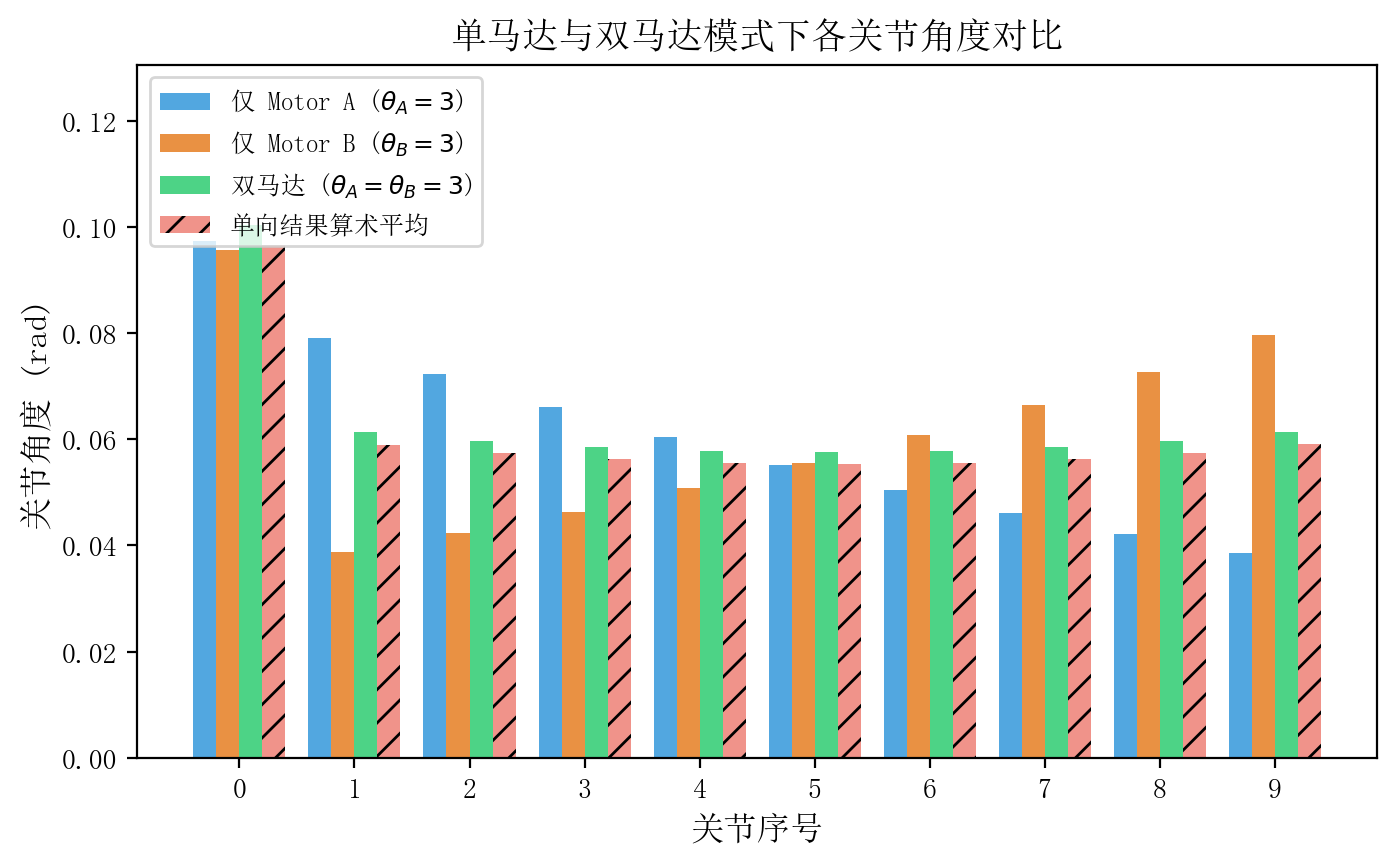
\includegraphics[width=0.78\textwidth]{figures/single_vs_dual.png}
\caption{单马达与双马达模式下各关节角度对比（$\theta_A,\theta_B$ 单位：rad）。蓝色为仅 Motor A，橙色为仅 Motor B，绿色为双马达同向驱动，红色虚线为两个单向结果的简单算术平均。双驱动结果介于两者之间且不与简单平均重合，体现了 Schur 补交叉耦合效应。}
\label{fig:single_vs_dual}
\end{figure}

工况 (a) 下，仅靠近 Motor A 侧的关节获得显著弯曲，关节角度沿 $\mathbf{S}_A^{\text{(paper)}}$ 方向分布。工况 (b) 呈现相反趋势。工况 (c) 的结果由 Schur 补公式精确求解。值得强调的是，工况 (c) 的关节角并非两个单向结果的简单平均——由于式\,\eqref{eq:schur_scalars} 中交叉项 $b$ 的存在，$\mathbf{R}_A$ 与 $\mathbf{R}_B$ 之间产生耦合效应，使得双马达结果在某些关节上偏向单向结果中较小的一方。若用 $(\mathbf{S}_A^{\text{(paper)}} + \mathbf{S}_B^{\text{(paper)}}) \cdot \sigma$ 近似双马达响应，则会高估中间关节的弯曲幅度。

\paragraph{实验 B：SDAS 与经典自适应协同模型对比}

实验 B 旨在说明 SDAS 模型在方法论上的核心改进。固定 $\sigma = 5$\,rad，变化 $\sigma_f \in [-2, 2]$\,rad，分别用 SDAS 模型和项目早期版本中的经典自适应协同模型（需额外构建 $\mathbf{R}_f$ 矩阵）计算关节角度。

\begin{figure}[htbp]
\centering
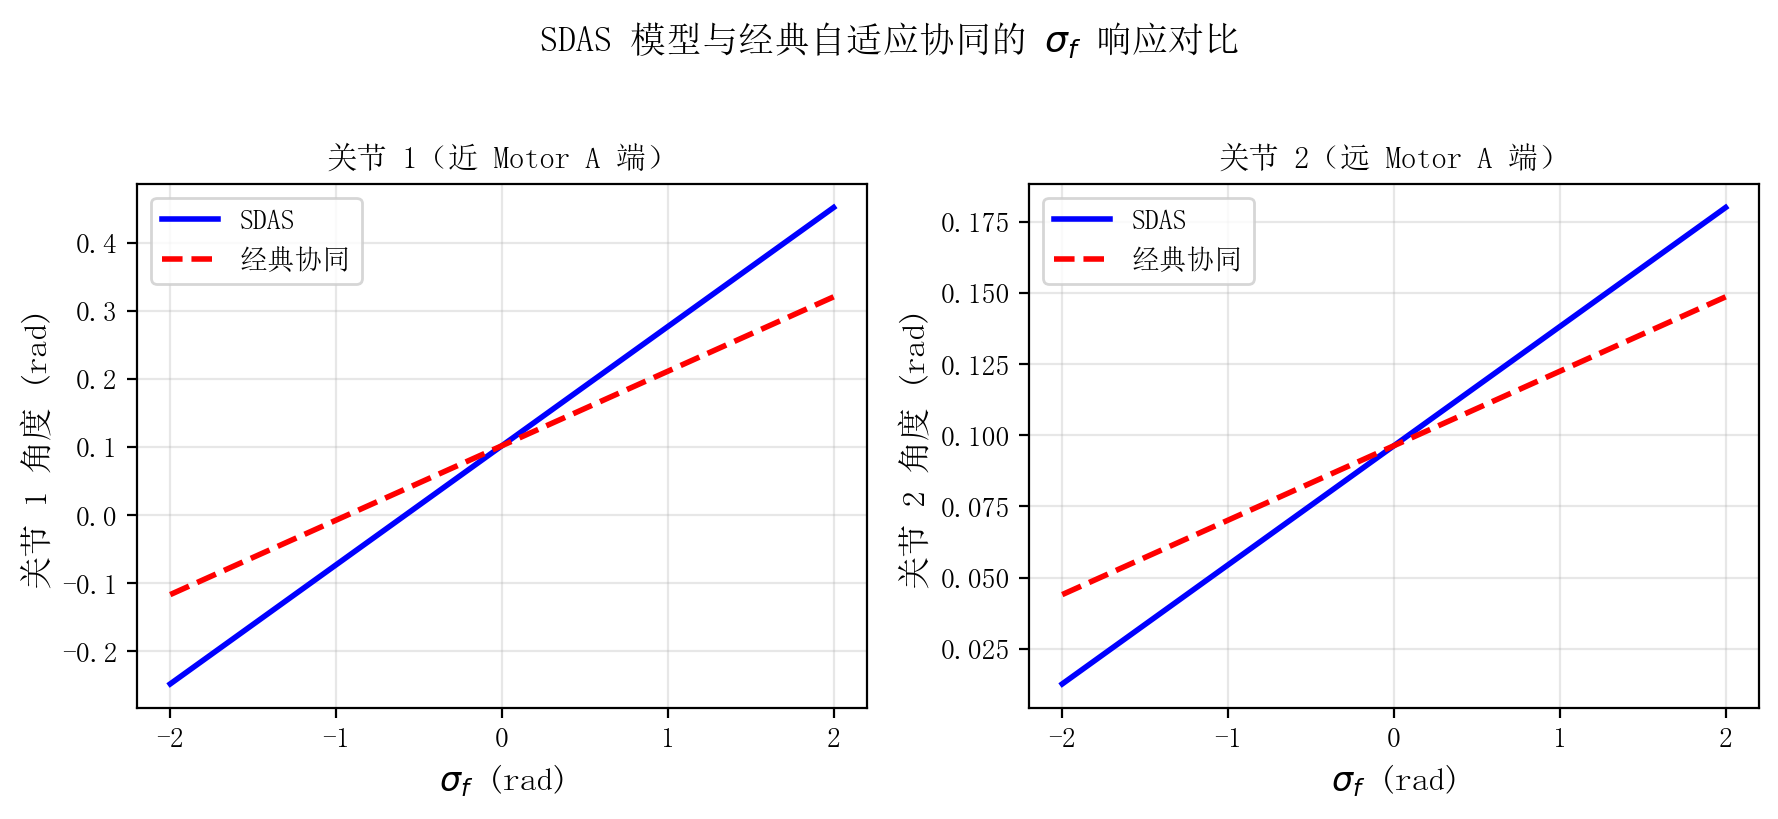
\includegraphics[width=0.78\textwidth]{figures/sdas_vs_classic.png}
\caption{SDAS 模型与经典自适应协同模型的 $\sigma_f$ 响应对比。横坐标为 $\sigma_f$（单位：rad），纵坐标为关节角度（单位：rad）。左图为关节 1 响应，右图为关节 2 响应。SDAS 模型（实线）通过 $\mathbf{R}_A \neq \mathbf{R}_B$ 自然产生非对称响应，无需显式 $\mathbf{R}_f$ 矩阵。}
\label{fig:sdas_vs_classic}
\end{figure}

经典自适应协同模型在 $\mathbf{R}$ 之外需要额外引入 $\mathbf{R}_f$ 矩阵描述 $\sigma_f$ 模式下的传动行为，其构建依赖于静摩擦``冻结''阈值（默认 $5\%$）。当 $\mathbf{R}_A$ 与 $\mathbf{R}_B$ 接近对称时，该机制退化为零向量，且 $\mathbf{R}_f$ 对阈值取值高度敏感。由图\,\ref{fig:sdas_vs_classic} 可见，SDAS 模型在各 $\sigma_f$ 取值下均输出非对称的关节角度分布，且 $\sigma_f$ 从负到正变化时关节角度的变化方向与 $\mathbf{R}_A/\mathbf{R}_B$ 的衰减方向一致。这种非对称性完全源于 $\mathbf{R}_A$ 与 $\mathbf{R}_B$ 的路径衰减差异，无需任何额外可调参数。

\paragraph{动力学数值仿真验证}

实验 C 使用 \lstinline{scripts/run_numerical_simulation.py} 执行 Phase 2（完整动力学，含惯性与阻尼）仿真，以验证 SDAS 模型在时间连续输入下的动态响应特性。设定 $\sigma(t) = 5$\,rad 恒定，$\sigma_f(t)$ 按三段阶梯函数变化：$0 \to -2 \to +2$\,rad，每段持续 0.3\,s，总时长 0.9\,s。该输入模拟了先共模握紧、再差模偏向 Motor B 侧、最后差模偏向 Motor A 侧的完整操作序列。

由式\,\eqref{eq:sigma_to_theta} 可知，该输入序列对应 $\theta_A(t)$ 和 $\theta_B(t)$ 经历了三个不同的工作状态：$0 \le t < 0.3$\,s 时为对称双马达拉动（$\theta_A = \theta_B = 5$\,rad），$0.3 \le t < 0.6$\,s 时不对称（$\theta_A = 3$\,rad, $\theta_B = 7$\,rad），$0.6 \le t \le 0.9$\,s 时不对称方向对调。

\begin{figure}[htbp]
\centering
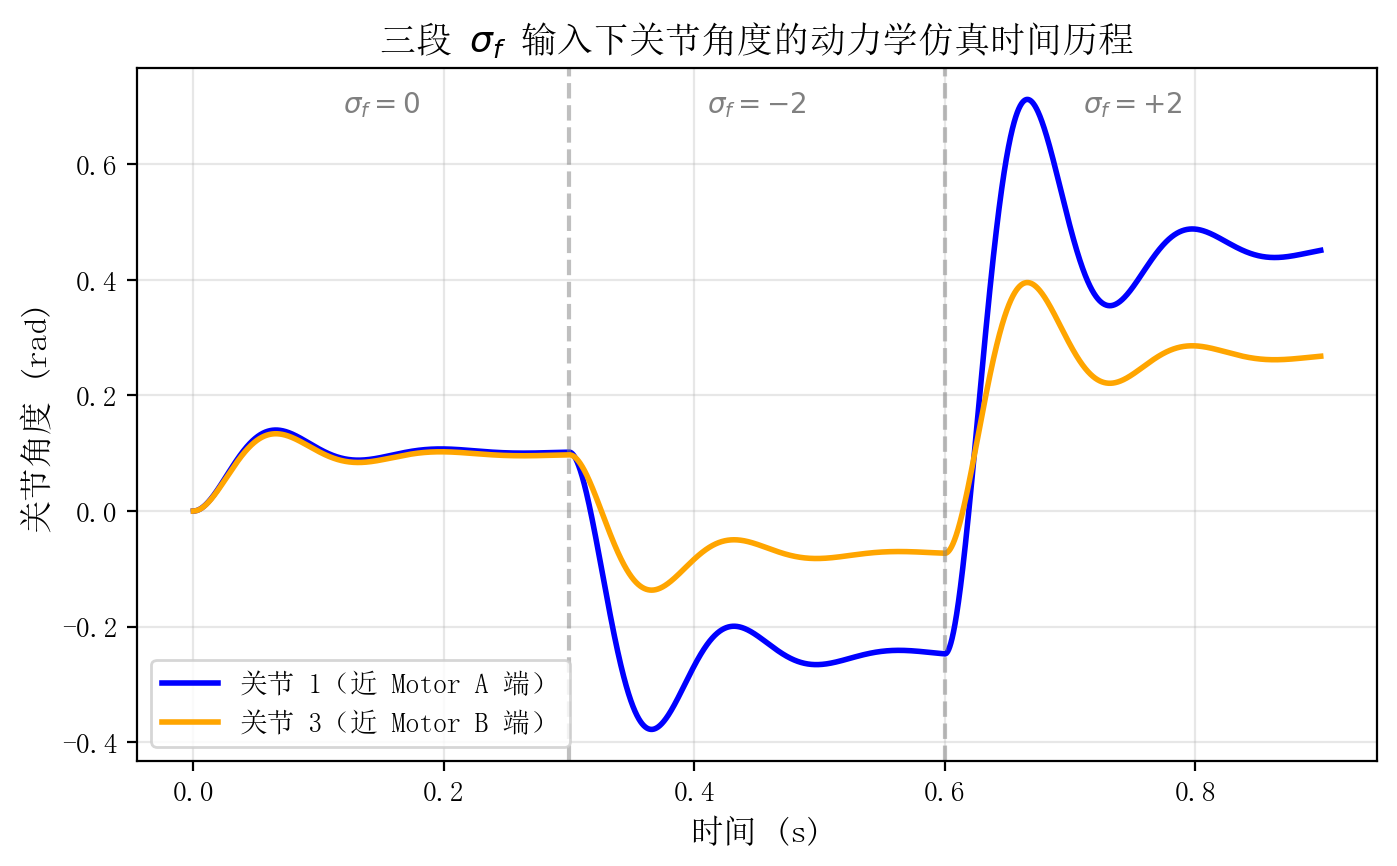
\includegraphics[width=0.78\textwidth]{figures/three_phase_simulation.png}
\caption{三段 $\sigma_f$ 输入下关节角度的动力学仿真时间历程。$\sigma_f$ 在 $t=0.3$\,s 和 $t=0.6$\,s 处阶跃切换。蓝色实线为关节 1（靠近 Motor A），橙色实线为关节 3（靠近 Motor B）。关节角度连续光滑过渡，无振荡或跳变。}
\label{fig:three_phase}
\end{figure}

图\,\ref{fig:three_phase} 展示了两组代表性关节的角度时间历程。关节 1（靠近 Motor A）在 $\sigma_f$ 从 0 切换至 $-2$ 时弯曲量减小，从 $-2$ 切换至 $+2$ 时弯曲量增大；关节 3（靠近 Motor B）的响应规律相反。这正是 $\mathbf{R}_A \neq \mathbf{R}_B$ 在时域中的直接体现。

在 $\sigma_f$ 发生阶跃的两个时刻（$t=0.3$\,s 和 $t=0.6$\,s），关节角度曲线连续且光滑，未出现任何不连续跳变或数值振荡。这表明 SDAS 求解器仅涉及矩阵乘法运算，其输出自然随时间连续变化，在动力学仿真中具有良好的数值稳定性。同时，动力学仿真中惯性项和阻尼项的存在使角度过渡更为平滑（相较纯运动学映射），且存在可观测的响应延迟——这是物理惯性的自然体现。

\paragraph{验证结论}

三组实验共同验证了 SDAS 模型的关键特性：(a) 约束选择策略物理正确，Schur 补公式精确描述了双马达耦合效应；(b) 通过 $\mathbf{R}_A/\mathbf{R}_B$ 的自然非对称性替代 $\mathbf{R}_f$ 概念，参数更简洁、物理含义更清晰；(c) 在三段式连续输入下关节角度响应连续光滑，数值稳定性优良，满足实时交互与动力学仿真的要求。


\subsubsection{小结}
\label{sec:summary}

本节系统地介绍了 SDAS 模型的软件实现方法，涵盖从数据结构设计、传动矩阵计算、约束求解器实现到交互式仿真环境构建的完整技术路线。总结起来，SDAS 模型的软件实现具有以下关键特征。

\textbf{基于 $\mathbf{R}_A$、$\mathbf{R}_B$ 的自然非对称性取消了 $\mathbf{R}_f$ 概念。} 经典自适应协同模型需要引入额外的静摩擦冻结参数构建 $\mathbf{R}_f$ 矩阵，SDAS 模型以 Capstan 摩擦导致的路径依赖衰减自然产生 $\mathbf{R}_A \neq \mathbf{R}_B$，从而在无需额外参数的前提下实现二维协同空间控制。

\textbf{状态依赖的约束选择策略。} 根据电机的激活状态自动切换求解公式：单马达拉动时使用单向公式，双马达同时拉动时使用 Schur 补公式。松弛钳位逻辑确保腱绳只能传递拉力这一物理事实被严格遵循，状态切换平滑自然。

\textbf{与 MuJoCo 的高效集成。} 通过 URDF 导出、空间最近邻关节映射和回调函数机制，SDAS 求解器被嵌入 MuJoCo 物理引擎的主循环。四滑块互联动接口实现了 $\theta_A/\theta_B$ 与 $\sigma/\sigma_f$ 两种控制模式间的无缝切换。

\textbf{支持动力学数值仿真验证。} 通过对 $\sigma_f$ 阶跃输入的动力学 Phase 2 仿真，验证了 SDAS 模型在时域中的连续响应能力和数值稳定性。

计算效率方面，单次 \lstinline{solve_motors()} 调用仅涉及若干标量与向量的线性组合操作，计算复杂度为 $\mathcal{O}(n^2)$（$n$ 为关节数），单次求解时间在 2--5\,$\mu$s 量级，完全满足 1\,kHz 的实时控制要求。三组数值实验的结果证实了 SDAS 模型在各工作状态下的行为正确性和数值稳定性，为后续章节中基于该模型的抓取实验与控制策略研究奠定了坚实的软件基础。

\end{document}
